\documentclass[a4paper, 12pt]{article}
\usepackage{geometry}
\usepackage{wrapfig}
\geometry{a4paper,
total={170mm,257mm},left=2cm,right=2cm,
top=2cm,bottom=2cm}

\usepackage{mathtext}
\usepackage{amsmath}
\usepackage[T2A]{fontenc}
\usepackage[utf8]{inputenc}
\usepackage[english,russian]{babel}
\usepackage{graphicx, float}
\usepackage{tabularx, colortbl}
\usepackage{caption}
\captionsetup{labelsep=period}

\newcommand{\parag}[1]{\paragraph*{#1:}}
\DeclareSymbolFont{T2Aletters}{T2A}{cmr}{m}{it}
\newcounter{Points}
\setcounter{Points}{1}
\newcommand{\point}{\arabic{Points}. \addtocounter{Points}{1}}
\newcolumntype{C}{>{\centering\arraybackslash}X}

\author{Калинин Даниил, Б01-110}
\date{11 апреля 2022}
\title{Лабораторная работа 2.4.1\\Определение теплоты испарения жидкости}

\begin{document}
\maketitle

\parag {Цель работы}
\begin{enumerate}
	\item измерение давления насыщенного пара жидкости при разной температуре;
	\item вычисление по полученным данным теплоты испарения с помощью уравнения Клапейрона–Клаузиуса.
\end{enumerate}

\parag {В работе используются}
термостат; герметический сосуд, заполненный исследуемой жидкостью; отсчетный микроскоп.

\parag {Теоритическая справка} ~\\
Испарением называется переход вещества из жидкого в газообразное состояние. При испарении с поверхности вылетают молекулы, образуя над ней пар. Для выхода из жидкости молекулы должны преодолеть силы молекулярного сцепления. Кроме того, при испарении совершается работа против внешнего давления $ P $, поскольку объем жидкости меньше объема пара. Не все молекулы жидкости способны совершить эту работу, а только те из них, которые обладают достаточной кинетической энергией. Поэтому переход части молекул в пар приводит к обеднению жидкости быстрыми молекулами, т.е. к ее охлаждению. Чтобы испарение проходило без изменения температуры, к жидкости нужно подводить тепло. Количество теплоты, необходимое для изотермического испарения одного моля жидкости при внешнем давлении, равном давлению ее насыщенных паров, называется молярной теплотой испарения (парообразования).

Теплоту парообразования жидкостей можно измерить непосредственно при помощи калориметра. Такой метод, однако, не позволяет получить точных результатов из-за неконтролируемых потерь тепла, которые трудно сделать малыми. В настоящей работе для определения теплоты испарения применен косвенный метод, основанный на формуле Клапейрона–Клаузиуса:

\begin{equation}\label{Kl-Kl}
\frac{dP}{dT}=\frac{L}{T\left(V_2-V_1\right)}.
\end{equation}

Здесь $ P $ -- давление насыщенного пара жидкости при температуре $ T $, $ T $ -- абсолютная температура жидкости и пара, $ L $ -- теплота испарения жидкости, $ V_2 $ -- объем пара, $ V_1 $ -- объем жидкости. Найдя из опыта $ dP/dT $, $ T $, $ V_2 $ и $ V_1 $, можно определить $ L $ путем расчета. Величины $ L $, $ V_2 $ и $ V_1 $ в формуле \eqref{Kl-Kl} должны относиться к одному и тому же количеству вещества; мы будем относить их к одному молю.

В нашем приборе измерения производятся при давлениях ниже атмосферного. В этом случае задача существенно упрощается.

При нашей точности опытов величиной $ V_1 $ в \eqref{Kl-Kl} можно пренебречь.

Обратимся теперь к $ V_2 $, которое в дальнейшем будем обозначать просто $ V $. Объем $ V $ связан с давлением и температурой уравнением Ван-дер-Ваальса:

\begin{equation}\label{VDV}
\left(P+\frac{a}{V^2}\right)\left(V-b\right)=RT.
\end{equation}

Из табличных данных следует, что $ b $ одного порядка с $ V_1 $. В уравнении Ван-дер-Ваальса величиной $ b $ следует пренебречь. Пренебрежение членом $ a/V^2 $ по сравнению с $ P $ вносит ошибку менее 3\%. При давлении ниже атмосферного ошибки становятся еще меньше. Таким образом, при давлениях ниже атмосферного уравнение Ван-дер-Ваальса для насыщенного пара мало отличается от уравнения Клапейрона. Положим поэтому

\begin{equation}\label{Volume}
V=\frac{RT}{P}.
\end{equation}

Подставляя \eqref{Volume} в \eqref{Kl-Kl}, пренебрегая $ V_1 $ и разрешая уравнение относительно $ L $, найдем

\begin{equation}\label{final}
L=\frac{RT^2}{P}\frac{dP}{dT}=-R\frac{d(\ln P)}{d(1/T)}.
\end{equation}

В нашем опыте температура жидкости измеряется термометром, давление пара определяется при помощи манометра, а производные $ dP/dT $ или $ d(\ln P)/d(1/T) $ находятся графически как угловой коэффициент касательной к кривой $ P(T) $ или соответственно к кривой, у которой по оси абсцисс отложено $ 1/T $, а по оси ординат $ \ln P $.

\parag {Экспериментальная установка}~\\

\begin{figure}
    \centering    
	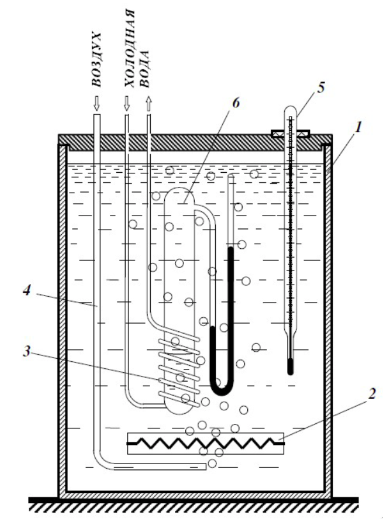
\includegraphics[width=10cm]{ust1.png}
	\caption{\textit{Схема первой установки}}
	\label{img1}
\end{figure}

Схема установки изображена на рисунке \ref{img1}. Наполненный водой резервуар 1 играет роль термостата. Нагревание термостата производится спиралью 2, подогреваемой электрическим током. Для охлаждения воды в термостате через змеевик 3 пропускается водопроводная вода. Вода в термостате перемешивается воздухом, поступающим через трубку 4. Температура воды измеряется термометром 5. В термостат погружен запаянный прибор 6 с исследуемой жидкостью. Над ней находится насыщенный пар (перед заполнением прибора воздух из него был откачан). Давление насыщенного пара определяется по ртутному манометру, соединенному с исследуемым объемом. Отсчет показаний манометра производится при помощи микроскопа.

На рисунке \ref{img2} приведена более полная схема такой же установки, но с использованием современного термостата. Установка включает термостат A, экспериментальный прибор B и отсчетный микроскоп C.

Экспериментальный прибор B представляет собой емкость 12, заполненную водой. В нее погружен запаянный прибор 13 с исследуемой жидкостью 14. Перед заполнением исследуемой жидкости воздух из запаянного прибора был удален, так что над жидкостью находится только её насыщенный пар. Давление пара определяется по ртутному манометру 15, соединенному с емкостью 13. Численная величина давления измеряется по разности показаний отсчетного микроскопа 16, настраиваемого последовательно на нижний и верхний уровни столбика ртути манометра. Показания микроскопа снимаются по шкале 17.

Описание прибора указывает на второе важное преимущество предложенного косвенного метода измерения $ L $ перед прямым. При непосредственном измерении теплоты испарения опыты нужно производить при неизменном давлении, и прибор не может быть запаян. При этом невозможно обеспечить такую чистоту и неизменность экспериментальных условий, как при нашей постановке опыта.

Описываемый прибор обладает важным недостатком: термометр определяет температуру термостата, а не исследуемой жидкости (или ее пара). Эти температуры близки друг к другу лишь в том случае, если нагревание происходит достаточно медленно. Убедиться в том, что темп нагревания не является слишком быстрым, можно, сравнивая результаты, полученные при нагревании и при остывании прибора. Такое сравнение необходимо сделать. Для ориентировки укажем, что температуру воды в калориметре следует менять не быстрее, чем на 1 $ ^\circ C $ в течение 1–3 минут.

\begin{figure}[H]
\begin{center}
		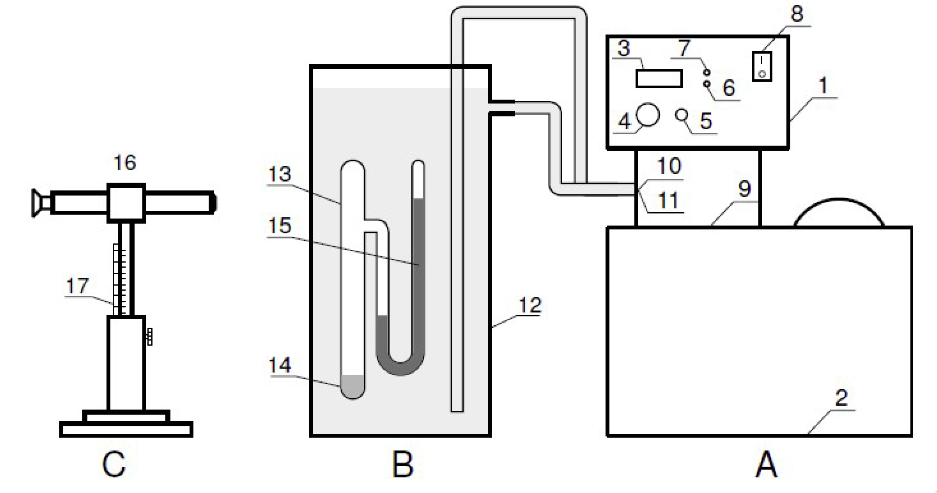
\includegraphics[width=15cm]{ust2.png}
\end{center}
	\caption{\textit{Схема второй установки}}
	\label{img2}
\end{figure}

\parag {Ход работы} ~\\


\point Запишем приборные погрешности: 
\begin{enumerate}
    \item Штангенциркуль: 0.05 мм.
    \item Термостат: 0.5 К
\end{enumerate}

\point Для определения теплоты парообразования воды измерим давление насыщенного пара при различных значениях температуры. Давление определяем при помощи ртутного манометра. При помощи штангенциркуля находим высоты $ h_1 $ и $ h_2 $ ртутных столбиков и по формуле

\begin{equation}\label{P}
    \Delta P = \rho g (h_1 - h_2)
\end{equation}  

находим давление насыщенного пара при определённой температуре. Результаты измерений заносим в таблицу \ref{tab:measures}.
    
При оценки погрешности измерения давления по формуле \eqref{P} следует использовать следующие соотношения:
\[ \sigma^2_{A\pm B} = \sigma^2_A+\sigma^2_B, \]
\[ \varepsilon^2_{A\cdot B} = \varepsilon^2_A+\varepsilon^2_B. \]
    
\point Занесём в таблицу \ref{tab:measures} значение давления насыщенного пара, вычисленное по формуле \eqref{P}.
    
\begin{table}[h]
    \centering
    \begin{tabular}{|c|c|c|c|c|c|c|c|c|}
        \cline{1-4} \cline{6-9}
        \multicolumn{4}{|c|}{Нагрев} &  & \multicolumn{4}{c|}{Охлаждение} \\ \cline{1-4} \cline{6-9}

        $ T $, К & $ h_1 $, мм & $ h_2 $, мм & $ \Delta P $, Па &  & $ T $, К & $ h_1 $, мм & $ h_2 $, мм & $ \Delta P $, Па \\ \cline{1-4} \cline{6-9} 
        296	& 7.3	& 9.29	& 265.31	& 	& 296	& 7.38	& 9.3	& 255.98	\\ \cline{1-4} \cline{6-9}
        298	& 7.2	& 9.36	& 287.98	& 	& 298	& 7.24	& 9.49	& 299.97	\\ \cline{1-4} \cline{6-9}
        300	& 7.19	& 9.52	& 310.64	& 	& 300	& 7.1	& 9.6	& 333.31	\\ \cline{1-4} \cline{6-9}
        302	& 7.05	& 9.68	& 350.64	& 	& 302	& 6.98	& 9.73	& 366.64	\\ \cline{1-4} \cline{6-9}
        304	& 6.88	& 9.84	& 394.63	& 	& 304	& 6.76	& 9.97	& 427.96	\\ \cline{1-4} \cline{6-9}
        306	& 6.7	& 10.19	& 465.29	& 	& 306	& 6.6	& 10.19	& 478.63	\\ \cline{1-4} \cline{6-9}
        308	& 6.59	& 10.34	& 499.96	& 	& 308	& 6.39	& 10.42	& 537.29	\\ \cline{1-4} \cline{6-9}
        310	& 6.24	& 10.59	& 579.95	& 	& 310	& 6.19	& 10.6	& 587.95	\\ \cline{1-4} \cline{6-9}
        312	& 5.98	& 10.81	& 643.95	& 	& 312	& 5.94	& 10.9	& 661.28	\\ \cline{1-4} \cline{6-9}
        314	& 5.68	& 11.16	& 730.60	& 	& 314	& 5.68	& 11.16	& 730.60	\\ \cline{1-4} \cline{6-9}
    \end{tabular}
    \caption{Измерение зависимости давления насыщенного пара от температуры жидкости}
    \label{tab:measures}
\end{table}
    
Используя перечисленные выше формулы, получаем, что погрешность измерения давления для каждого измерения составляет $ \sigma \approx 0.66 $ Па. ($ \varepsilon \approx 0,24 \% $). 
    
\point По данным из таблицы \ref{tab:measures} построим график зависимости давления насыщенного пара от температуры.

\begin{figure}
    \centering    
    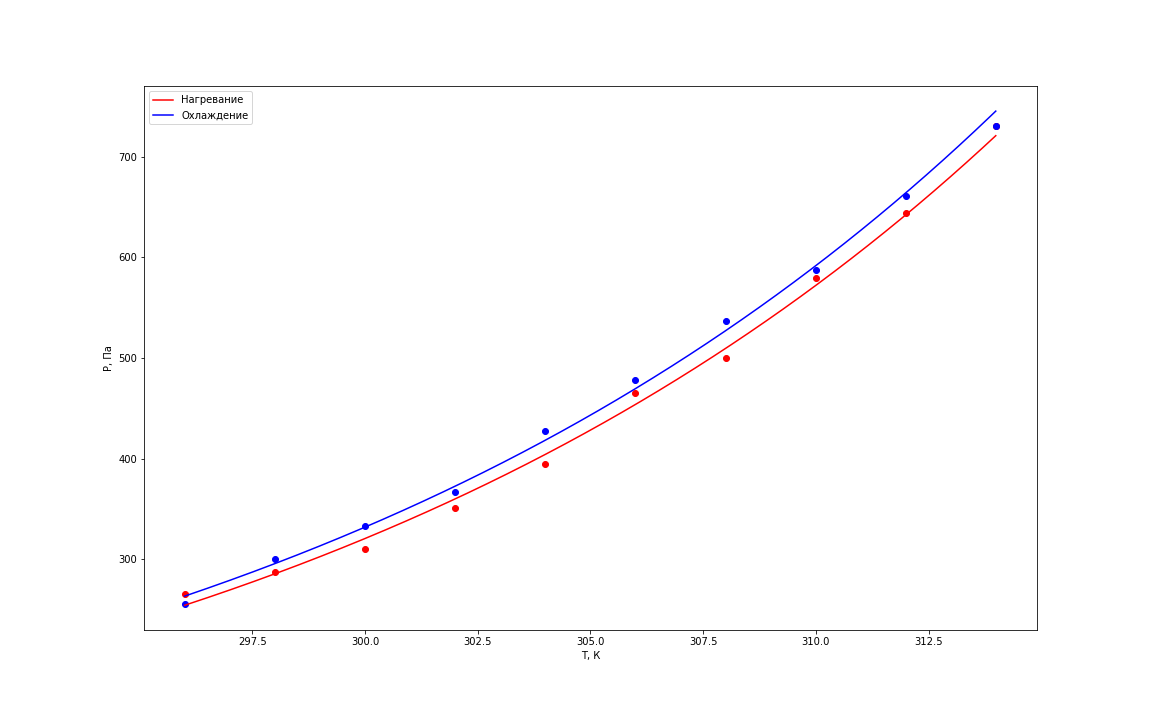
\includegraphics[width=18cm]{P_from_T.png}
    \caption{График зависимости P(T)}
    \label{P_from_T}
\end{figure}
    

\point Аппроксимируем методом наименьших квадратов полученные на этом участке температур зависимости функциями вида \[ P=ae^{bT}, \] где $ a $ и $ b $ -- неизвестные параметры. Используем следующие формулы:

\[ b = \frac{\langle \ln P \cdot T \rangle - \langle T \rangle \langle \ln P \rangle}{\langle T^2 \rangle - \langle T \rangle ^2},\]
\[ \ln a = \langle \ln P \rangle - b\langle T \rangle. \]

Случайные погрешности вычисления этих величин находим по следующим формулам:

\[ \sigma^\text{случ}_b = \sqrt{\frac{1}{N-2} \left(\frac{\left\langle\left(\ln P - \langle \ln P\right\rangle\right)^2 \rangle}{\left\langle\left(T - \langle T\right\rangle\right)^2 \rangle}\right)-b^2},\]
\[ \sigma^\text{случ}_{\ln a}=\sigma^\text{случ}_b\sqrt{\left\langle T^2 \right\rangle}. \]

\label{mnk}

Вкладом систематической погрешности в общую можно пренебречь в виду её малости по сравнению со случайной погрешностью определения коэффициентов. Поэтому будем считать, что \[ \sigma_b \approx \sigma^\text{случ}_b, \] \[ \sigma_{\ln a} \approx \sigma^\text{случ}_{\ln a}. \]

\point Полученные результаты заносим в таблицу \ref{tab:ab} и наносим зависимости на график.

\begin{table}[H]
	\centering
	\begin{tabular}{|c|c|c|c|c|}
		\hline
		Опыт & $ a \cdot 10^{-6}$, Па & $ \sigma_a \cdot 10^{-6}$, Па & $ b \cdot 10^{-2} $, К$ ^{-1} $ & $ \sigma_b \cdot 10^{-2} $, К$ ^{-1} $ \\ \hline
		нагрев      & 9.227 & 0.37 & 5.78 & 0,07 \\ \hline
		охлаждение  & 9.835  & 0.33 & 5.77 & 0,06 \\ \hline
	\end{tabular}
	\caption{Определение коэффициентов зависимости}
	\label{tab:ab}
\end{table}

\point Используя полученные результаты, можно получить формулу для производной давления по температуру: 
\begin{equation}\label{dpdt}
\frac{dP}{dT} = abe^{bT}.
\end{equation}
Подставляя \eqref{dpdt} в \eqref{final}, получаем:
\begin{equation}\label{newFinal}
L=\frac{RT^2ab}{P}e^{bT}.
\end{equation}

\point По полученным выше формулам вычисляем теплоту парообразования воды. Погрешность вычисления этой величины можно оценить по следующим формулам:
\[ \sigma_L = L\varepsilon_{\frac{dP}{dT}}, \]
\[ \sigma_{\frac{dP}{dT}} = \sqrt{\left(\frac{\partial\frac{dP}{dT}}{\partial a}\sigma_a\right)^2+\left(\frac{\partial\frac{dP}{dT}}{\partial b}\sigma_b\right)^2} \]

Полученные результаты заносим в таблицу \ref{tab:par}.

\begin{table}[h]
	\centering
	\begin{tabular}{|c|c|c|c|c|c|c|}
		\cline{1-3} \cline{5-7}
		\multicolumn{3}{|c|}{Нагрев} &  & \multicolumn{3}{c|}{Охлаждение} \\ \cline{1-3} \cline{5-7}

		$ T $, К & $ P $, Па & $ L $, $ \frac{\text{кДж}}{\text{моль}} $ &  & $ T $, К & $ P $, Па & $ L $, $ \frac{\text{кДж}}{\text{моль}} $ \\ \cline{1-3} \cline{5-7} 
        296	& 265.31	& 40.47	& 	& 296	& 255.98	& 43.37	\\ \cline{1-3} \cline{5-7}
        298	& 287.98	& 42.43	& 	& 298	& 299.97	& 42.11	\\ \cline{1-3} \cline{5-7}
        300	& 310.64	& 44.76	& 	& 300	& 333.31	& 43.11	\\ \cline{1-3} \cline{5-7}
        302	& 350.64	& 45.11	& 	& 302	& 366.64	& 44.58	\\ \cline{1-3} \cline{5-7}
        304	& 394.63	& 45.60	& 	& 304	& 427.96	& 43.44	\\ \cline{1-3} \cline{5-7}
        306	& 465.29	& 44.00	& 	& 306	& 478.63	& 44.18	\\ \cline{1-3} \cline{5-7}
        308	& 499.96	& 46.57	& 	& 308	& 537.29	& 44.76	\\ \cline{1-3} \cline{5-7}
        310	& 579.95	& 45.66	& 	& 310	& 587.95	& 46.51	\\ \cline{1-3} \cline{5-7}
        312	& 643.95	& 46.77	& 	& 312	& 661.28	& 47.02	\\ \cline{1-3} \cline{5-7}
        314	& 730.60	& 46.88	& 	& 314	& 730.60	& 48.38	\\ \cline{1-3} \cline{5-7}
        
	\end{tabular}
	\caption{Результаты вычисления теплоты парообразования}
	\label{tab:par}
\end{table}

\point Теперь построим зависимость $ \ln P $ от $ 1 / T $. Завимиость изображена на рисунке \ref{lnP_from_1_over_T}.

\begin{figure}
    \centering    
    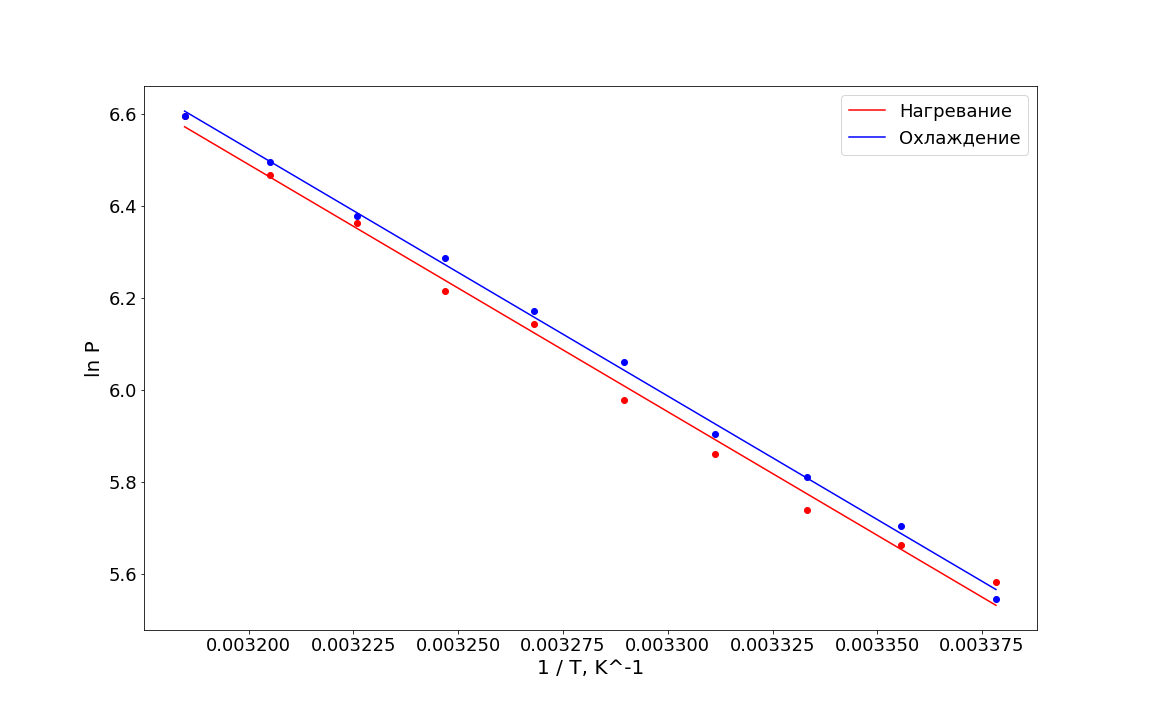
\includegraphics[width=18cm]{ln_p_from_1_over_T.png}
    \caption{График зависимости ln P(1/T)}
    \label{lnP_from_1_over_T}
\end{figure}

С помощью формул метода наименьших квадратов, описанных выше, вычислим значение и погрешность определения коэффициента $ \displaystyle \frac{d(\ln P)}{d(1/T)} $. Таким образом, получаем

\[ \left(\frac{d(\ln P)}{d(1/T)}\right)_\text{нагр} = \left(-5375\pm38\right)\text{ К}, \]

\[ \left(\frac{d(\ln P)}{d(1/T)}\right)_\text{охл} = \left(-5373\pm42\right)\text{ К}. \]

По формуле \eqref{final} вычисляем теплоту парообразования. Получаем:

\[ L_\text{нагр} = \left(44.725 \pm 0,5\right) \text{ } \frac{\text{кДж}}{\text{моль}}, \]
\[ L_\text{охл} = \left(44.709 \pm 0.7\right) \text{ } \frac{\text{кДж}}{\text{моль}}. \]


\parag {Заключение} ~\\
В ходе выполнения работы:

\begin{enumerate}
	\item была исследована зависимость давления насыщенных паров от давления жидкости;
	\item были вычислены теплоты парообразования жидкости для различных температур двумя разными способами.
\end{enumerate}

Кроме этого, теплота парообразования была определена при помощи графика зависимости $ \ln P $ от $ 1/T $. По результатам этих измерений получили:

\[L_\text{нагр} = \left(2.484 \pm 0.04\right) \text{ } \frac{\text{кДж}}{\text{кг}} \quad (\varepsilon = 1.6 \%), \]
\[ L_\text{охл} = \left(2.483 \pm 0.02\right) \text{ } \frac{\text{кДж}}{\text{кг}} \quad (\varepsilon = 1.2 \%).  \]


Нетрудно заметить, что данные, полученные при помощи двух различных методов, хорошо согласуются друг с другом.

Сравним полученные данные с табличными. Из табличных данных:

\[ L = 2.3 \text{ } \frac{\text{кДж}}{\text{кг}}. \]

Отсюда видно, что полученные данные с хорошей точностью совпадают с табличными. В тоже время, у этого метода высокая случайная погрешность вычисления.

\end{document}
